\documentclass[11pt]{article}
\ifdefined\pdfinfoomitdate\pdfinfoomitdate=1\fi
\ifdefined\pdftrailerid\pdftrailerid{}\fi
\ifdefined\pdfsuppressptexinfo\pdfsuppressptexinfo=15\fi
\usepackage[T1]{fontenc}
\usepackage{lmodern}
\usepackage[margin=1in]{geometry}
\usepackage{amsmath,amssymb,amsthm,mathtools}
\usepackage{microtype}
\usepackage{enumitem}
\usepackage{booktabs}
\usepackage{xcolor}
\usepackage{tikz}
\usetikzlibrary{arrows.meta,positioning,calc,patterns}
\usepackage[numbers,sort&compress]{natbib}
\usepackage[hyphens]{url}
\usepackage{hyperref}
\hypersetup{colorlinks=true,linkcolor=blue!45!black,citecolor=blue!45!black,
 urlcolor=blue!45!black,pdfauthor={OpenAI},
 pdftitle={Turn-Based Stochastic Mean-Payoff Games in Deterministic Quasipolynomial Time}}
\numberwithin{equation}{section}
\newtheorem{theorem}{Theorem}[section]
\newtheorem{lemma}[theorem]{Lemma}
\newtheorem{proposition}[theorem]{Proposition}
\newtheorem{corollary}[theorem]{Corollary}
\theoremstyle{definition}
\newtheorem{definition}[theorem]{Definition}
\theoremstyle{remark}
\newtheorem{remark}[theorem]{Remark}
\newcommand{\R}{\mathbb R}
\newcommand{\Z}{\mathbb Z}
\newcommand{\N}{\mathbb N}
\newcommand{\Q}{\mathbb Q}
\newcommand{\E}{\mathbb E}
\newcommand{\Prb}{\mathbb P}
\newcommand{\one}{\mathbf 1}
\newcommand{\val}{\operatorname{val}}
\newcommand{\MP}{\operatorname{MP}}
\newcommand{\cL}{\mathcal L}
\newcommand{\supp}{\operatorname{supp}}
\newcommand{\idtext}[1]{\begingroup\urlstyle{same}\nolinkurl{#1}\endgroup}
\DeclareMathOperator{\den}{den}
\setlist[enumerate]{leftmargin=*,itemsep=4pt}
\setlength{\emergencystretch}{2em}
\title{Turn-Based Stochastic Mean-Payoff Games\\in Deterministic Quasipolynomial Time}
\author{OpenAI}
\date{October 5, 2026}
\begin{document}
\maketitle
\begin{abstract}
We give a uniform deterministic quasipolynomial-time algorithm for finite
turn-based stochastic mean-payoff games with signed integer rewards and
rational chance-transition probabilities encoded in binary. It computes
exactly the vertices of nonnegative value, including value zero, for the
expectation of the pathwise liminf mean payoff. The algorithm uses exact
rational arithmetic and $2^{O((\log(L+2))^2)}$ bit operations, where $L$
is the complete binary input length.
\end{abstract}
\section{Introduction}
\label{sec:introduction}

Mean-payoff games ask how two players can control the long-run average
reward of an infinite play. In the stochastic version, some transitions
are chosen by chance. This combines strategic choice with the possibility
of moving between regions having different long-run rewards. The input
may describe very small transition probabilities and very large rewards
with only a few binary digits, so an algorithm whose cost depends on
their magnitudes need not be efficient in the input length.

\subsection{The problem and the result}

An instance consists of a finite directed multigraph $G=(V,E)$ with
$V=\{1,\ldots,n\}$, $n\ge1$, and at least one outgoing edge at every
vertex. The vertex set is partitioned as
\[
 V=V_{\max}\sqcup V_{\min}\sqcup V_{\mathrm{ch}}.
\]
Each edge $e$ has an integer reward $w(e)$. At a vertex of $V_{\max}$,
Max chooses the next edge; at a vertex of $V_{\min}$, Min chooses it;
at a vertex $i\in V_{\mathrm{ch}}$, the next edge is drawn from a
prescribed rational probability distribution $p_i$ on the outgoing
edges. Rewards and the numerators and positive denominators of the
probabilities are encoded in binary. The graph and all edge data are
listed explicitly. Loops, parallel edges, zero probabilities, and
unreduced fractions are permitted.

Both players observe the complete finite history, including traversed
edges, and may use arbitrary behavioral strategies with private
randomness. Chance draws have the prescribed conditional law at the
current vertex. A pure positional strategy chooses one outgoing edge at
each vertex of its player, independently of the preceding history.
For a play $\pi=(X_0,e_0,X_1,e_1,\ldots)$ define
\[
 \MP_w(\pi)=\liminf_{T\to\infty}\frac1T\sum_{t=0}^{T-1}w(e_t),
 \qquad
 \val(i)=\sup_\sigma\inf_\tau
           \E_{i,\sigma,\tau}[\MP_w].
\]
Here $\sigma$ and $\tau$ range over Max's and Min's behavioral
strategies, respectively. The expectation is taken after the pathwise
lower limit. If $L$ is the complete binary input length, the decision
problem is to output the set
\[
                         U=\{i\in V:\val(i)\ge0\}.
\]

\begin{theorem}
\label{thm:main}
There are a uniform deterministic Turing machine and an absolute constant
$C$ such that, on every valid input described above, the machine outputs
exactly $U$ in at most
\[
                       2^{C(\log_2(L+2))^2}
\]
bit operations. The bound includes input reading, exact rational
arithmetic, and output. Vertices of value zero are included.
\end{theorem}

\subsection{Historical context}
\label{subsec:history}

Shapley introduced stochastic games with positive stopping probabilities
and characterized their values by a contraction operator
\cite{Shapley1953}. Gillette considered the undiscounted, long-run
average objective \cite{Gillette1957}; Liggett and Lippman supplied
the classical stationary-strategy theorem for perfect-information
time-average games \cite{LiggettLippman1969}. The relation between
discounting and long-run optimization is also classical. Blackwell
showed in finite dynamic programming that one stationary policy is
optimal for every discount factor sufficiently close to one
\cite{Blackwell1962}. Rational discounted values provide the
corresponding stabilization mechanism for perfect-information
stochastic games; see, for example, Gimbert and Zielonka
\cite[Theorem~3]{GimbertZielonka2010}.

The computational problem connects several familiar classes of games.
A simple stochastic game is a finite turn-based reachability game in
which chance chooses fairly between two successors. Condon placed its
threshold problem in $\mathrm{NP}\cap\mathrm{coNP}$
\cite{Condon1992}, and Ludwig gave a randomized subexponential
algorithm \cite{Ludwig1995}. Zwick and Paterson developed
pseudopolynomial algorithms for deterministic mean-payoff games and
a reduction to simple stochastic games \cite{ZwickPaterson1996}.
Andersson and Miltersen later proved polynomial-time Turing
equivalences among computing values and optimal strategies in
simple stochastic, stochastic mean-payoff, and stochastic
discounted-payoff games, with numerical parameters---including the
discount factor---given in binary
\cite[Theorem~1]{AnderssonMiltersen2009}.
Randomized strategy-improvement algorithms have
subexponential expected bounds \cite{Zwick2026}. A different line
obtains pseudopolynomial bounds when the number of random positions
is fixed \cite{BorosEtAl2019,AllamigeonEtAl2025}. Numerical reward
and denominator parameters in such bounds distinguish them from a
bound in the complete binary input length. Deterministic
quasipolynomial algorithms have also been obtained for simple
stochastic games of bounded treewidth \cite{ChatterjeeEtAl2023}.

Theorem~\ref{thm:main} also gives a deterministic quasipolynomial
algorithm for deciding whether the reachability value of a simple
stochastic game is at least $1/2$. Make the target absorbing, with
reward $+1$ on its self-loop, and give every other edge reward $-1$;
any other terminal vertex receives a self-loop of reward $-1$.
For every strategy pair the pathwise mean payoff is
$2\one_{\{\text{target is reached}\}}-1$.
Its expectation is twice the reachability probability minus one,
so taking the strategy extrema proves the reduction. The transformation
increases the input length by at most a constant factor.

An explicit small discount is only one part of the present algorithm.
Andersson and Miltersen already bounded a sufficient discount using
determinant coefficients and polynomial sign stabilization
\cite[Lemma~1]{AnderssonMiltersen2009}; Gaubert, Grand-Cl\'ement,
and Katz give sharper bounds on Blackwell optimality thresholds
\cite{GaubertGrandClementKatz2025}.
Hansen, Miltersen, and Zwick proved that strategy iteration is
strongly polynomial when the discount factor is fixed
\cite{HansenMiltersenZwick2013}. The dependence of their bound on
the inverse distance of that factor from one does not yield a
polynomial bound in its binary encoding. Here the discount has
polynomial bit length, and a recursive comparison algorithm controls
the cost of locating its fixed point.

For games without chance vertices, a deterministic quasipolynomial
algorithm in the complete binary input length is given in
\citet[Theorem~1.1]{OpenAI2026Deterministic}. Its simultaneous labeling
construction is the direct predecessor of the method used here. We
extend that construction to discounted operators, so that chance
transitions enter through the same order and translation properties
as player choices.

\subsection{The proof and its main ideas}

The first part of the proof replaces the mean-payoff problem by one
discounted fixed point. For $0<u<1$, the discounted map takes the maximum,
minimum, or chance average of $u w(e)+(1-u)t_j$ over edges $e:i\to j$.
It is a contraction and has a unique fixed point $v(u)$. An explicit
integer $H$, of polynomial binary length, gives a nonzero-value gap of
at least $1/H$ and a discount $\lambda$ for which
$\|v(\lambda)-\val\|_\infty\le1/(16H)$. Section~\ref{sec:discount}
proves these estimates by elementary bounds on the rational functions
of a fixed positional pair. Its gain and bias then give pathwise
guarantees against every behavioral opponent. This establishes the
payoff convention used here directly.

Finding the discounted fixed point by ordinary contraction iteration
would take a number of steps depending on $1/\lambda$, which can be
exponential in the input length. The second part of the proof treats
any monotone map $F:\R^n\to\R^n$ satisfying
\[
             F(t+c\one)=F(t)+\gamma c\one,
             \qquad 0<\gamma<1.
\]
In an integer box, a subsolution is an integer vector $y$ satisfying
$F_i(y)\ge y_i$ at coordinates above the lower face; a supersolution
satisfies the reverse inequality at coordinates below the upper face.
A subsolution close to an upper face requires a plus label there,
while a supersolution close to a lower face requires a minus label.
The procedure assigns each coordinate a positive mass for each sign.
Its guarantee holds simultaneously for all comparison vectors whose
coordinates away from the opposite face have total mass at most one.

Section~\ref{sec:labeling} adapts the two-pass pivot and mass-reweighting
method of \citet[Sections~4--5]{OpenAI2026Deterministic}.
The crucial translations have a fixed sign: subsolutions move downward
and supersolutions upward. The discounted translation identity preserves
their required inequalities, allowing comparison vectors in a large box
to be used in smaller recursive boxes. Two pivot passes then arrange a
redistribution of the masses that keeps the required comparisons valid.
At each recursive call, at most one child leaves both mass vectors
unchanged. Every other child increases each product of a coordinate's
two masses by a fixed factor. Starting from uniform masses, only
$O(\log(n+1))$ such choices are possible along a path, even when the
coordinate range is exponentially large.

The final part explains why these boundary labels suffice to find the
fixed point. After scaling, we place an integer subsolution $Y$ and an
integer supersolution $Z$ on opposite sides of it, with $Z-Y$ uniformly
small. Neither vector is computed. A label excluding one comparison
vector from a boundary strip permits that boundary to move inward while
retaining both. Section~\ref{sec:application} shrinks the enclosing box
in this way, and the value gap converts the final approximation into
the exact nonnegative-value set.

The reusable part of the argument is the labeling procedure: its
correctness uses monotonicity and the scalar translation identity,
and does not inspect the graph or the transition probabilities. The
two-sided integer comparison vectors provide the link from that
procedure to a discounted game. Quantitative discounting supplies the
required accuracy, while the recursion determines the deterministic
quasipolynomial running time.

Throughout, vector inequalities, extrema, and integer rounding are
coordinatewise, and $\one$ denotes the all-ones vector. The proof uses
only exact arithmetic.

\section{A quantitative discount reduction}
\label{sec:discount}

We first reduce the sign of each mean-payoff value to an approximation of
one discounted fixed point. The reduction needs two quantitative facts:
nonzero values are separated from zero, and a discount of polynomial bit
length approximates every value more accurately than this separation.
We prove both facts directly, including the identification of the limiting
discounted value with the expected pathwise lower average.

The discounted fixed-point method originates in Shapley's work
\cite{Shapley1953}. Our argument for a single positional pair at all small
discounts is a quantitative version of the eventual-optimality principle
introduced by Blackwell for finite Markov decision processes
\cite{Blackwell1962}; stationary optimality for perfect-information
stochastic games with limiting-average payoffs was established by Liggett
and Lippman \cite{LiggettLippman1969}. Quantitative thresholds for
small-discount optimality are studied further in
\cite{GaubertGrandClementKatz2025}. The estimates and the payoff
convention needed here are proved below.

Let $n=|V|$, and define
\begin{equation}
\begin{split}
 W&=\max\bigl(1,\max_{e\in E}|w(e)|\bigr),\\
 Q&=\prod_{\substack{e\text{ outgoing from}\\i\in V_{\mathrm{ch}}}}
       \operatorname{den}(p_i(e)),\\
 A_0&=n!\,[Q(3+W)]^n,
 \qquad H=(W+4)A_0,
 \qquad \lambda_0=\frac1{32H^2}.
\end{split}
\label{eq:discount-parameters}
\end{equation}
Here $W,Q,A_0,H$ are positive integers. The denominator in the product
defining $Q$ is the positive denominator supplied in the input; the
fractions need not be reduced. An empty product is one.
The explicit input gives $n=O(L)$ and $\log Q,\log W=O(L)$, because
the denominator and reward bits are included in $L$. Therefore
\[
 \log H=O\!\left(n\bigl(\log(n+1)+\log Q+\log(W+3)\bigr)\right)
        =O((L+2)^2),
\]
so $\lambda_0$ has polynomial bit length.

For $0<u<1$, define $f_u:\R^V\to\R^V$ by taking at vertex $i$ the
maximum, minimum, or prescribed chance average of
\begin{equation}
                 u w(e)+(1-u)t_j,
                 \qquad e:i\longrightarrow j,
\label{eq:discount-edge}
\end{equation}
according as $i$ belongs to Max, Min, or Chance. This map is monotone and
is a contraction in the maximum norm, with constant $1-u$. Indeed, each
expression in \eqref{eq:discount-edge} changes by at most
$(1-u)\|t-t'\|_\infty$, and taking an extremum or an average preserves
that bound. Its iterates from zero converge, because the successive
differences decrease geometrically. Their limit is the unique fixed
point, denoted $v(u)$. Since $f_u$ preserves $[-W,W]^V$,
\begin{equation}
                       \|v(u)\|_\infty\le W.
\label{eq:discount-bound}
\end{equation}

\begin{theorem}[Quantitative discount reduction]
\label{thm:discount}
For every game in the input class, there are vectors $G,\psi\in\R^V$
and a pure positional strategy pair $(\sigma^*,\tau^*)$ whose selected
edges attain the extrema defining $f_u(v(u))$ for every
$0<u\le1/(2H)$. Moreover,
\begin{equation}
                 v_i(u)=G_i+u\psi_i+O(u^2)
                 \qquad(u\downarrow0).
\label{eq:gain-bias-expansion}
\end{equation}
For every start vertex $i$ and every behavioral opposing strategy,
\begin{equation}
 \E_{i,\sigma^*,\tau}[\operatorname{MP}_w]\ge G_i,
 \qquad
 \E_{i,\sigma,\tau^*}[\operatorname{MP}_w]\le G_i.
\label{eq:gain-strategy-bounds}
\end{equation}
Consequently $G_i=\val(i)$. Each $G_i$ is rational with a representation
whose denominator has absolute value at most $A_0$, and
\begin{equation}
 \begin{gathered}
 |G_i|\le W,
 \qquad G_i\ne0\ \Longrightarrow\ |G_i|\ge\frac1H,\\
 |v_i(\lambda_0)-G_i|\le\frac1{16H}.
 \end{gathered}
\label{eq:discount-gap-error}
\end{equation}
\end{theorem}

The proof has an algebraic part and a probabilistic part. Rational
functions first give a pair that works for every sufficiently small
discount, together with its limiting gain $G$ and first-order term
$\psi$. We then use these two vectors to control individual plays
against arbitrary behavioral opponents.

\subsection{A positional pair valid for all small discounts}

Temporarily fix a pure positional pair: one outgoing edge at each Max
and Min vertex. Let $P$ be its row-stochastic transition matrix and let
$r_i$ be its expected one-step reward at $i$. At a chance vertex the
transition probabilities of parallel edges are added in $P$, whereas
their possibly different rewards are averaged in $r$. The pair's
discounted equations are
\begin{equation}
                       x(u)=u r+(1-u)P x(u).
\label{eq:pair-discount-equations}
\end{equation}
The matrix $I-(1-u)P$ is invertible for $0<u<1$: a vector in its kernel
would satisfy $\|x\|_\infty\le(1-u)\|x\|_\infty$. The corresponding
affine contraction preserves $[-W,W]^V$, so its solution satisfies
$\|x(u)\|_\infty\le W$.

The determinant argument follows the rational-function sign method
of Andersson and Miltersen \cite[Lemma~1]{AnderssonMiltersen2009};
we derive all coefficient bounds in the input parameters above.
For a polynomial $a$, write $\|a\|_{\mathrm{coef}}$ for the sum of
the absolute values of its coefficients. This norm is subadditive and
submultiplicative. Every entry of $QP$ and $Qr$ is an integer. Cramer's
rule therefore gives integer polynomials $N_i,D$ with
\begin{equation}
 x_i(u)=\frac{N_i(u)}{D(u)},
 \qquad D(u)=\det\bigl(Q(I-(1-u)P)\bigr).
\label{eq:discount-cramer}
\end{equation}
Each entry of the matrix defining $D$ has coefficient norm at most $3Q$.
The replacing column defining $N_i$ is $Qu r$, whose entries have
coefficient norm at most $QW$. Expanding each determinant over its $n!$
permutations gives
\begin{equation}
 \|D\|_{\mathrm{coef}}\le A_0,
 \qquad \|N_i\|_{\mathrm{coef}}\le A_0.
\label{eq:discount-polynomial-bound}
\end{equation}

Whether this pair's chosen edge is optimal at a player vertex $i$ is
determined by comparisons with every outgoing edge $e:i\to j$. Each
comparison is the sign of
\begin{equation}
 x_i(u)-u w(e)-(1-u)x_j(u)
   =\frac{N_i(u)-u w(e)D(u)-(1-u)N_j(u)}{D(u)}.
\label{eq:discount-edge-comparison}
\end{equation}
The numerator has coefficient norm at most $(3+W)A_0\le H$.

To control these signs, let $a$ be any nonzero integer polynomial with
$\|a\|_{\mathrm{coef}}\le H$. Factoring its lowest power of $u$ gives
$a(u)=u^\ell(c+u q(u))$, where $c$ is a nonzero integer. For
$0<u\le1/(2H)$,
\[
                   |u q(u)|\le Hu\le\tfrac12<|c|.
\]
Thus the sign of $a(u)$ throughout this interval is the sign of its
lowest nonzero coefficient. This observation applies to both the
numerator and denominator in \eqref{eq:discount-edge-comparison};
the denominator is nonzero there by invertibility. Every edge comparison
therefore has a constant sign or vanishes identically on the interval.

Now choose attaining edges in the maximum and minimum defining
$f_{\lambda_0}(v(\lambda_0))$. They give a pure positional pair
$(\sigma^*,\tau^*)$, and its linear solution at $\lambda_0$ equals
$v(\lambda_0)$. Since $\lambda_0\le1/(2H)$, all edge inequalities
that hold at $\lambda_0$ continue to hold for every $0<u\le1/(2H)$.
For each such $u$, the pair's linear solution is consequently a fixed
point of $f_u$, hence equals $v(u)$. The pair is needed for the proof;
the algorithm need not compute it.

\subsection{The rational gain and its approximation error}

Use the polynomials of the pair just selected. Let $\ell$ be the lowest
nonzero degree of $D$. Boundedness of $N_i(u)/D(u)$ as $u\downarrow0$
implies that $u^\ell$ also divides each $N_i$. Define
$\widehat D=D/u^\ell$ and $\widehat N_i=N_i/u^\ell$.
Their coefficient norms satisfy \eqref{eq:discount-polynomial-bound},
and $\widehat D(0)$ is a nonzero integer. The quotient is analytic at
zero, so it has the expansion \eqref{eq:gain-bias-expansion}, with
\begin{equation}
                         G_i=\frac{\widehat N_i(0)}{\widehat D(0)}.
\label{eq:rational-gain}
\end{equation}
The bound \eqref{eq:discount-bound} gives $|G_i|\le W$. The displayed
denominator has magnitude at most $A_0$, and its numerator is an
integer. Thus $G_i\ne0$ implies $|G_i|\ge1/A_0\ge1/H$.

The same coefficient bounds also control the approximation error.
The polynomial $\widehat N_i-G_i\widehat D$ has constant coefficient
zero and coefficient norm at most $(1+W)A_0$. For
$0<u\le1/(2H)$, the tail of $\widehat D$ has magnitude at most
$A_0u\le1/2$, so $|\widehat D(u)|\ge1/2$. It follows that
\begin{equation}
 |v_i(u)-G_i|
   \le 2(1+W)A_0u
   \le 2Hu.
\label{eq:uniform-discount-error}
\end{equation}
At $u=\lambda_0$, this is the error claimed in
\eqref{eq:discount-gap-error}.

It remains to identify $G_i$ with the mean-payoff value. The gain
controls which transitions can persist, and the coefficient $\psi$
then controls the rewards on those transitions. For a selected player
edge $e:i\to j$, substitution of \eqref{eq:gain-bias-expansion} into
the discounted equation gives
\begin{equation}
               G_i=G_j,
               \qquad \psi_i=w(e)+\psi_j-G_j.
\label{eq:selected-gain-bias}
\end{equation}
At a chance vertex, the corresponding identities are
\begin{equation}
 \begin{split}
 G_i&=\sum_{e:i\to j}p_i(e)G_j,\\
 \psi_i&=\sum_{e:i\to j}p_i(e)\bigl(w(e)+\psi_j-G_j\bigr).
 \end{split}
\label{eq:chance-gain-bias}
\end{equation}
At a Min vertex, the inequality
$v_i(u)\le u w(e)+(1-u)v_j(u)$ for an arbitrary outgoing edge first
gives $G_i\le G_j$. If $G_i=G_j$, subtracting this common constant,
dividing by $u$, and letting $u\downarrow0$ gives
\begin{equation}
                  \psi_i\le w(e)+\psi_j-G_j.
\label{eq:min-gain-bias}
\end{equation}
At a Max vertex, the gain inequality and, when the gains agree, the
bias inequality both reverse.

\subsection{From one-step inequalities to pathwise payoffs}

We use two elementary facts about adapted processes. Fixing a selected
strategy will give the gain along a play one-sided conditional drift.
The first lemma shows that the gain then becomes constant, so only
gain-preserving player moves can persist and the bias inequalities
apply. The second lemma shows that the centered contributions at chance
vertices have vanishing averages.

\begin{lemma}[Finite-valued submartingales]
\label{lem:finite-submartingale}
Let $(Z_t)_{t\ge0}$ be adapted to a filtration $(\mathcal F_t)_{t\ge0}$
and take values in a fixed finite subset of $\R$. If
$\E[Z_{t+1}\mid\mathcal F_t]\ge Z_t$ for every $t$, then $Z_t$ is
eventually constant almost surely. Its eventual value $Z_\infty$
satisfies $\E Z_\infty\ge\E Z_0$.
\end{lemma}

\begin{proof}
Add a constant to make $Y_t=Z_t+c$ nonnegative. Conditional expectation
and the assumed drift give
\[
 \begin{split}
 \E[Y_{t+1}^2-Y_t^2]
 &=\E[(Y_{t+1}-Y_t)^2]
   +2\E\!\left[Y_t\,\E[Y_{t+1}-Y_t\mid\mathcal F_t]\right]\\
 &\ge\E[(Y_{t+1}-Y_t)^2].
 \end{split}
\]
Summing and using boundedness shows that
$\E\sum_{t\ge0}(Y_{t+1}-Y_t)^2<\infty$. The sum is therefore finite
almost surely. If there is more than one possible value, let $\Delta>0$
be the minimum distance between distinct values. Every change contributes
at least $\Delta^2$ to the sum, so only finitely many changes occur.
The singleton case is immediate. Finally, $\E Z_t\ge\E Z_0$ for all
$t$, and bounded convergence gives the claimed expectation inequality.
\end{proof}

\begin{lemma}[Averages of bounded martingale differences]
\label{lem:bounded-martingale-average}
Let $(\mathcal F_t)_{t\ge0}$ be a filtration. Suppose $D_t$ is
$\mathcal F_{t+1}$-measurable,
$\E[D_t\mid\mathcal F_t]=0$, and $|D_t|\le c$ for a fixed finite
constant $c$. Then $T^{-1}\sum_{t<T}D_t\to0$ almost surely.
\end{lemma}

\begin{proof}
For $s<t$, conditioning on $\mathcal F_t$ gives $\E[D_sD_t]=0$.
Hence $\E[(\sum_{t<T}D_t)^2]\le Tc^2$. Chebyshev's inequality at
$T=j^2$ gives, for every $\varepsilon>0$,
\[
 \mathbb P\!\left(\left|\frac1{j^2}\sum_{t<j^2}D_t\right|>
          \varepsilon\right)
 \le\frac{c^2}{\varepsilon^2j^2}.
\]
The sum over $j$ is finite. The probability that one of these events
occurs after index $m$ is at most the tail of this sum, which tends to
zero. Applying this argument to $\varepsilon=1,1/2,1/3,\ldots$ proves
convergence along squares on a single event of probability one.
For $j^2\le T<(j+1)^2$, the additional partial sum has magnitude at
most $c(2j+1)$. Dividing by $T\ge j^2$ extends convergence to every
$T$.
\end{proof}

\begin{proof}[Completion of the proof of Theorem~\ref{thm:discount}]
Fix a start vertex $i$, fix Max to $\sigma^*$, and let Min use an
arbitrary behavioral strategy. Write $X_t$ for the vertex before the
edge $e_t$ is traversed, and let $\mathcal F_t$ be the sigma-field
generated by the complete observed history through $X_t$. At a chance
vertex the conditional law of $e_t$ is the prescribed distribution.
At a player vertex it is the
distribution induced by that player's strategy, including any private
randomness.

The process $G_{X_t}$ has nonnegative conditional drift. A selected Max
edge preserves $G$ by \eqref{eq:selected-gain-bias}; every Min edge
weakly increases $G$; and the first identity in
\eqref{eq:chance-gain-bias} gives zero drift at a chance vertex.
Lemma~\ref{lem:finite-submartingale} gives an eventual value
$G_\infty$ with
\begin{equation}
                         \E G_\infty\ge G_i.
\label{eq:gain-limit-expectation}
\end{equation}

Define the one-step residual and its chance part by
\[
 R_t=w(e_t)+\psi_{X_{t+1}}-\psi_{X_t}-G_{X_t},
 \qquad
 D_t=\mathbf 1_{\{X_t\in V_{\mathrm{ch}}\}}R_t.
\]
These random variables are uniformly bounded because the arena is
finite. At a chance vertex, the two identities in
\eqref{eq:chance-gain-bias} imply
\[
 \E[R_t\mid\mathcal F_t]
   =\sum_{e:X_t\to j}p_{X_t}(e)(w(e)+\psi_j)
      -\psi_{X_t}-G_{X_t}=0.
\]
Outside chance vertices $D_t=0$. Thus
$\E[D_t\mid\mathcal F_t]=0$, and
Lemma~\ref{lem:bounded-martingale-average} gives
$T^{-1}\sum_{t<T}D_t\to0$ almost surely.

After $G_{X_t}$ has become constant, every traversed nonchance edge
preserves $G$. Its residual is zero at Max vertices by
\eqref{eq:selected-gain-bias}, and nonnegative at Min vertices by
\eqref{eq:min-gain-bias}. The nonchance residuals are therefore
nonnegative except for a finite initial segment. Consequently
\[
                    \liminf_{T\to\infty}\frac1T\sum_{t<T}R_t\ge0
                    \qquad\text{almost surely}.
\]
Telescoping the bias terms gives
\begin{equation}
 \frac1T\sum_{t<T}w(e_t)
   =\frac1T\sum_{t<T}G_{X_t}
     +\frac1T\sum_{t<T}R_t
     +\frac{\psi_{X_0}-\psi_{X_T}}{T}.
\label{eq:gain-bias-telescoping}
\end{equation}
The first average tends to $G_\infty$, and the last term tends to zero.
Hence $\operatorname{MP}_w\ge G_\infty$ almost surely. Taking
expectations and using \eqref{eq:gain-limit-expectation} proves the
first inequality in \eqref{eq:gain-strategy-bounds}.

For the second inequality, fix Min to $\tau^*$ and let Max be arbitrary.
Now $-G_{X_t}$ has nonnegative conditional drift. The same finite-valued
lemma yields an eventual gain $G_\infty$ with $\E G_\infty\le G_i$.
The chance residuals still have average zero. At Min vertices the
selected edges have residual zero; at Max vertices an edge preserving
$G$ has nonpositive residual by the reversed version of
\eqref{eq:min-gain-bias}. Thus the nonchance residuals are eventually
nonpositive, and \eqref{eq:gain-bias-telescoping} gives
\[
             \limsup_{T\to\infty}\frac1T\sum_{t<T}w(e_t)
                    \le G_\infty
                    \qquad\text{almost surely}.
\]
This also bounds the pathwise lower average. Taking expectations proves
the second inequality in \eqref{eq:gain-strategy-bounds}.

Max can therefore guarantee $G_i$, and Min can guarantee that the payoff
is at most $G_i$, so $\val(i)=G_i$. The payoffs and gain limits in these
expectation comparisons are bounded. The argument permits each opposing
history-dependent distribution and establishes the expected-liminf
convention directly.
\end{proof}

\section{Simultaneous labeling for discounted monotone maps}
\label{sec:labeling}

We now construct the labels that will permit a box to shrink while
retaining the integer comparison vectors around the discounted fixed
point.  The construction depends only on order and on the response to
a common translation.  We therefore work in the following abstract
setting: $n\ge1$ and $F:\R^n\to\R^n$ satisfy
\begin{equation}
 t\le t'\ \Longrightarrow\ F(t)\le F(t'),\qquad
 F(t+c\one)=F(t)+\gamma c\one
 \quad(t\in\R^n,\ c\in\R),\qquad 0<\gamma<1.
 \label{eq:label-map}
\end{equation}
All vector inequalities, minima, maxima, and floors in this section
are coordinatewise.  The algorithm uses $F$ only by evaluating
$\lfloor F(t)\rfloor$ at integer vectors $t$.

The two pivot passes and subsequent mass change adapt the simultaneous
labeling construction of
\cite[Sections~4--5]{OpenAI2026Deterministic}.  Here the operator has
the discounted translation rule in Equation~\eqref{eq:label-map}.
The proof below establishes the required labeling theorem directly;
the signs of the witness translations are what make that adaptation
possible.

\subsection{Witnesses and the labeling guarantee}

An input consists of $A\in\Z^n$, a width
\begin{equation}
 D=h2^d,\qquad 128\le h\le255,\quad h,d\in\Z,\quad d\ge0,
 \label{eq:label-width}
\end{equation}
and positive rational mass vectors $a,b\in\mathbb Q_{>0}^n$.
Write $u=A+D\one$, $P=D/32$, and
$a(S)=\sum_{i\in S}a_i$, $b(S)=\sum_{i\in S}b_i$ for
$S\subseteq\{1,\ldots,n\}$.  The representation in
Equation~\eqref{eq:label-width} is unique.  Its short range of
mantissas will later allow small relative decreases in the width.

\begin{definition}[Witnesses and claims]
\label{def:label-witness}
An integer vector $y\in[A,u]$ is a \emph{subsolution in the box} if
\[
 F_i(y)\ge y_i\quad\text{for every }i\in S_y,
 \qquad S_y=\{i:y_i>A_i\}.
\]
It is a \emph{plus witness} if also $a(S_y)\le1$; its claims are
the indices $i$ for which $y_i\ge u_i-P$.

An integer vector $z\in[A,u]$ is a \emph{supersolution in the box} if
\[
 F_i(z)\le z_i\quad\text{for every }i\in S_z,
 \qquad S_z=\{i:z_i<u_i\}.
\]
It is a \emph{minus witness} if also $b(S_z)\le1$; its claims are
the indices $i$ for which $z_i\le A_i+P$.
The sets $S_y,S_z$ are the respective supports.  A witness is
\emph{relevant} if it has at least one claim.
\end{definition}

Every claim belongs to its witness's support, since $0<P<D$.
The output must respect all these claims simultaneously, although
the algorithm is not given any witness and does not search for one.

\begin{theorem}[Recursive simultaneous labeling]
\label{thm:labeling}
Let $F:\R^n\to\R^n$ satisfy Equation~\eqref{eq:label-map}.
There is a terminating deterministic procedure $\cL(A,D,a,b)$,
using exact evaluations of $\lfloor F(t)\rfloor$ for $t\in\Z^n$
and integer and rational arithmetic, with the following guarantee.
For every input as in Equation~\eqref{eq:label-width} and
Definition~\ref{def:label-witness}, its output
$\ell\in\{+,-\}^n$ satisfies
\[
 \begin{aligned}
 y_i\ge A_i+D-P&\ \Longrightarrow\ \ell_i=+
       &&\text{for every plus witness }y,\\
 z_i\le A_i+P&\ \Longrightarrow\ \ell_i=-
       &&\text{for every minus witness }z.
 \end{aligned}
\]
\end{theorem}

The existence of a labeling will already follow from the finite box
iteration below.  The purpose of the recursive construction is to
obtain such labels with the controlled branching and decreasing rank
of Lemma~\ref{lem:label-rank}, replacing dependence on the numerical
width by dependence on its exponent.

\begin{lemma}[Comparison and a finite box iteration]
\label{lem:label-comparison}
Every subsolution $y$ and supersolution $z$ in the same box satisfy
$y\le z$.  Starting at $t^0=u$, the iteration
\begin{equation}
 t^{m+1}=T(t^m),\qquad
 T(t)=\min\{u,\max\{A,\lfloor F(t)\rfloor\}\},
 \label{eq:label-floor}
\end{equation}
stops at a vector $t^*$ after at most $nD+1$ evaluations of $T$.
For every such pair $y,z$ one has $y\le t^*\le z$.
\end{lemma}

\begin{proof}
If $m=\max_j(y_j-z_j)>0$, choose $i$ with $y_i-z_i=m$.
Since $y_i>z_i\ge A_i$ and $z_i<y_i\le u_i$, both defining
inequalities apply at $i$.  Monotonicity and the common translation
rule give
\[
 m\le F_i(y)-F_i(z)
   \le F_i(z+m\one)-F_i(z)=\gamma m,
\]
a contradiction.

The map $T$ preserves the finite integer box and is monotone.
Moreover $T(u)\le u$, so induction gives $t^{m+1}\le t^m$.
Each changing step decreases the nonnegative integer
$\sum_i(t_i^m-A_i)$ by at least one.  Its initial value is $nD$,
which proves the termination bound, including the final unchanged
step.

For an integer $y\in[A,u]$, the subsolution condition is equivalent
to $y\le T(y)$.  Indeed, when $y_i>A_i$, the latter inequality is
equivalent to $y_i\le\lfloor F_i(y)\rfloor$, and at the other
coordinates it is automatic.  If $y$ is a subsolution, induction
gives $y\le t^m$: from $y\le t^m$ one obtains
$y\le T(y)\le T(t^m)=t^{m+1}$.  Thus $y\le t^*$.
The fixed point $t^*=T(t^*)$ is itself a subsolution, and the
comparison principle gives $t^*\le z$ for every supersolution $z$.
\end{proof}

\subsection{The recursive procedure}

A \emph{centered call} of even width $r$ at an integer pivot $k$
means the call $\cL(k-(r/2)\one,r,a',b')$ with the indicated
masses.  All calls use the same map $F$.  In a nonbase call set
\begin{equation}
 c=A+\frac D2\one,\qquad M=\frac D8,\qquad
 q=\frac D{128},\qquad p=\frac q{32}=\frac D{4096}.
 \label{eq:label-scales}
\end{equation}
The pivot will stay between $c-M\one$ and $c+M\one$.
The two passes use narrow centered boxes to identify some labels
directly and arrange the remaining witnesses so that the later mass
change preserves their admissibility. The downward pass preserves
the plus masses, and the upward pass preserves the minus masses.
A final wider centered call supplies the signs used to change both
mass vectors.

\medskip
\noindent\textbf{Procedure $\cL(A,D,a,b)$.}
Execute the first applicable base case.  If neither applies, execute
Steps~3--6 in order.
\begin{enumerate}
\item \textbf{Mass base case.}
If $a_i b_i>1$ for every $i$, return $+$ at $i$ when $b_i>1$,
and return $-$ otherwise.

\item \textbf{Width base case.}
If $d<12$, compute $t^*$ by Equation~\eqref{eq:label-floor}.
Return $+$ at $i$ when $t_i^*>A_i+D/2$, and return $-$ otherwise.

\item \textbf{Downward pass.}
Initialize $k=c$.  Make a centered width-$q$ call at $k$ with
masses $(a,\frac43 b)$, and use its labels to update all coordinates
simultaneously by
\begin{equation}
 k_i^{\mathrm{new}}=
 \begin{cases}
  \max\{c_i-M,k_i-p\},&\text{if the child labels }i\text{ by }-,\\
  k_i,&\text{if the child labels }i\text{ by }+.
 \end{cases}
 \label{eq:label-down-update}
\end{equation}
Replace $k$ by $k^{\mathrm{new}}$ and repeat until an update leaves
the pivot unchanged.  Denote this last pivot by $k^{\downarrow}$ and set
\begin{equation}
 I_- =\{i:k_i^{\downarrow}<c_i-P\}.
 \label{eq:label-minus-override}
\end{equation}

\item \textbf{Upward pass.}
Start at $k=k^{\downarrow}$.  Make a centered width-$q$ call at $k$
with masses $(\frac43 a,b)$, and update simultaneously by
\begin{equation}
 k_i^{\mathrm{new}}=
 \begin{cases}
  \min\{c_i+M,k_i+p\},&\text{if the child labels }i\text{ by }+,\\
  k_i,&\text{if the child labels }i\text{ by }-.
 \end{cases}
 \label{eq:label-up-update}
\end{equation}
Replace $k$ by $k^{\mathrm{new}}$ and repeat until an unchanged
update.  Denote the last pivot by $k^f$ and set
\begin{equation}
 I_+ =\{i:k_i^f>c_i+P\}.
 \label{eq:label-plus-override}
\end{equation}

\item \textbf{Provisional labels and new masses.}
Make a centered width-$D/2$ call at $k^f$ with masses $(a,b)$.
For its output $\ell^0$, define
\begin{equation}
 (\bar a_i,\bar b_i)=
 \begin{cases}
  (\frac45 a_i,\frac85 b_i),&\ell_i^0=+,\\[1mm]
  (\frac85 a_i,\frac45 b_i),&\ell_i^0=-.
 \end{cases}
 \label{eq:label-reweight}
\end{equation}

\item \textbf{Continuation and overrides.}
Call $\cL(A,D,\bar a,\bar b)$.  In its output replace the signs
on $I_-$ by $-$ and those on $I_+\setminus I_-$ by $+$.
Return this label vector.
\end{enumerate}

Each pass includes the final child call whose update changes nothing.
That call will certify a mass inequality at the stopped pivot.  All
coordinates in one update use the same old pivot and the same child
output; there is no order-dependent coordinate update.

The purpose of the passes is the following mass property. For every
witness with a claim outside its own override set---$I_+$ for a plus
witness and $I_-$ for a minus witness---the coordinates in its support
whose provisional labels match its sign will have total mass greater
than $3/4$. Here mass means $a$-mass for a plus witness and $b$-mass
for a minus witness. Its original total mass is at most one, so
Step~5 will leave its new total mass below
\[
                  \frac85-\frac45\cdot\frac34=1.
\]
It will therefore remain a witness for the continuation in the
unchanged box. At the same time, every product $a_i b_i$ is multiplied
by $32/25$. We first use this product growth to prove termination;
the subsequent witness analysis proves the stated mass property and
hence correctness.

\begin{lemma}[Valid boxes and bounded passes]
\label{lem:label-mechanics}
Every child input is valid and its box lies inside its parent's box.
If the child calls terminate, each pivot pass makes at most
$1024n+1$ calls.  The width base case makes at most
$522240n+1$ evaluations of $\lfloor F\rfloor$.
\end{lemma}

\begin{proof}
In a nonbase call $d\ge12$, so $c,M,q,p$ and the half-widths
$q/2,D/4$ are integral.  The centered widths have the allowed
representations $q=h2^{d-7}$ and $D/2=h2^{d-1}$.
The pivot caps keep $c-M\one\le k\le c+M\one$, and a centered
box has width $r\le D/2$.  Its boundaries satisfy
\[
 k-\frac r2\one\ge A+\frac D8\one\ge A,
 \qquad
 k+\frac r2\one\le A+\frac{7D}8\one\le u.
\]
The continuation uses the same box.  All masses remain positive
rationals.

Every pivot coordinate lies on the grid of spacing $p$ through
$c_i$, because $M/p=512$ is integral.  In a changing update some
coordinate moves by $p$; each coordinate is monotone during a pass
and travels at most $2M$, hence moves at most $1024$ times.
There are at most $1024n$ changing updates, followed by one
unchanged update.  Finally, $d<12$ implies
$D\le255\cdot2^{11}=522240$, so the width bound follows from
Lemma~\ref{lem:label-comparison}.
\end{proof}

The continuation preserves the width, so width reduction alone does
not prove termination.  The mass products provide the missing
measure.  Define
\begin{equation}
 \mu(a,b)=\min_i a_i b_i,\qquad \rho=\frac{32}{25},\qquad
 B(\mu)=\min\{j\in\Z_{\ge0}:\rho^j\mu>1\}.
 \label{eq:label-budget}
\end{equation}
This integer is used only in the proof, not computed by the procedure.

\begin{lemma}[Rank and branching]
\label{lem:label-rank}
The procedure terminates.  At a nonbase call every child has smaller
rank $d+B(\mu(a,b))$.  There is exactly one child preserving $B$,
the provisional call, and it decreases $d$ by one.  There are at most
$2048n+3$ other children; each decreases $B$ by at least one and
does not increase $d$.
\end{lemma}

\begin{proof}
At a nonbase call $B(\mu)>0$, since otherwise the mass base case
would apply.  Whenever $\mu'\ge\rho\mu$, the definition gives
$B(\mu')\le B(\mu)-1$.  Both pivot passes multiply every mass
product by $4/3\ge\rho$.  The continuation multiplies every mass
product by $(4/5)(8/5)=\rho$, independently of the provisional
label.  These children reduce $B$ and preserve or reduce $d$.
Only the provisional call keeps the masses; it halves the width
and reduces $d$ by one.  This proves the rank assertion.

Induction on the nonnegative rank proves termination.  The base cases
are finite by their definitions and Lemma~\ref{lem:label-mechanics}.
At a nonbase call every child terminates by induction, and the bound
on each pivot pass then applies.  The number of children decreasing
$B$ is at most $2(1024n+1)+1=2048n+3$.
\end{proof}

\subsection{Translating a witness into a centered box}

To analyze the labels, we follow an arbitrary parent witness through
the centered calls.  Translation places its largest deviation from
the pivot at one boundary of the child box; clipping removes
coordinates far below that largest deviation.  The surviving support
will identify the mass forced near the largest deviation when a
pivot pass stops.

Fix a nonbase input and a pivot $k\in[c-M\one,c+M\one]$.
For a relevant plus witness $y$, define its \emph{peak} and
\emph{gaps} by
\begin{equation}
 s_y(k)=\max_i(y_i-k_i),\qquad
 g_i^y(k)=s_y(k)-(y_i-k_i).
 \label{eq:label-plus-gaps}
\end{equation}
For a relevant minus witness $z$, put
\begin{equation}
 s_z(k)=\max_i(k_i-z_i),\qquad
 g_i^z(k)=s_z(k)-(k_i-z_i).
 \label{eq:label-minus-gaps}
\end{equation}
The gaps are nonnegative integers and at least one gap is zero.
The following lemma handles both signs, including the inequalities
introduced by the discount factor.

\begin{lemma}[Translation and clipping]
\label{lem:label-translation}
Let $r\in\{q,D/2\}$ and let $y$ or $z$ be a relevant witness
of the parent box.  Define, according to its sign,
\begin{equation}
 \begin{aligned}
 y'_i&=\max\{k_i-r/2,\ y_i-s_y(k)+r/2\},\\
 z'_i&=\min\{k_i+r/2,\ z_i+s_z(k)-r/2\}.
 \end{aligned}
 \label{eq:label-translation}
\end{equation}
The resulting vector is an integer subsolution or supersolution,
respectively, in the centered width-$r$ box.  Its support is exactly
$\{i:g_i(k)<r\}$, which is contained in the parent's support.
It claims every index with $g_i(k)\le r/32$.  It is a witness
for that child whenever its support has mass at most one for the
child's mass vector of the corresponding sign.
\end{lemma}

\begin{proof}
A parent claim gives, in either case,
\begin{equation}
 s(k)\ge D/2-M-P=11D/32.
 \label{eq:label-peak-lower}
\end{equation}
Outside the parent support one has $y_i=A_i$ or $z_i=u_i$.
The corresponding deviation is at most $-D/2+M=-3D/8$,
so its gap is at least $23D/32>D/2$.  Such an index cannot
belong to $\{i:g_i(k)<r\}$.

Before clipping, the two expressions on the right of
Equation~\eqref{eq:label-translation} are
\[
 k_i+r/2-g_i^y(k),\qquad
 k_i-r/2+g_i^z(k),
\]
respectively.  They lie on the correct side of the far boundary;
clipping at the other boundary puts the vector in the child box.
These expressions also show directly that the support is exactly
the set of gaps strictly below $r$, and that every gap at most
$r/32$ gives a claim.

For the plus case let $t=-s_y(k)+r/2<0$, where the strict sign
follows from Equation~\eqref{eq:label-peak-lower} and $r/2\le D/4$.
One has $y'\ge y+t\one$.  At an index in the child support,
equality holds in that coordinate, and the parent subsolution
inequality applies.  Therefore
\[
 F_i(y')\ge F_i(y+t\one)=F_i(y)+\gamma t
          \ge y_i+t=y'_i,
\]
using $\gamma t\ge t$.  For the minus case let
$t=s_z(k)-r/2>0$.  Now $z'\le z+t\one$, with coordinatewise
equality on the child support, and
\[
 F_i(z')\le F_i(z+t\one)=F_i(z)+\gamma t
          \le z_i+t=z'_i,
\]
using $\gamma t\le t$.  Thus the required inequalities survive
both translation and clipping.  The stated mass condition is
exactly the remaining condition for being a child witness.
\end{proof}

\subsection{What the two pivot passes enforce}

We prove correctness by induction on the rank from
Lemma~\ref{lem:label-rank}.  For the remainder of this subsection,
fix a nonbase call and assume that all its children satisfy
Theorem~\ref{thm:labeling}.  Witnesses, supports, and claims refer
to the parent input unless stated otherwise.

In each pass, the sign whose masses are unchanged protects its own
peak: coordinates close enough to that peak must receive its sign
and remain stationary.  The opposite sign has its masses multiplied
by $4/3$.  At the final unchanged update, any witness of that sign
with a claim outside its override set must consequently have mass greater than
$3/4$ near its peak.  The next two lemmas make these statements
precise.

\begin{lemma}[The downward pass]
\label{lem:label-down}
For every relevant plus witness $y$, the peak $s_y(k)$ is constant
throughout the downward pass and at most $D/2$.  No plus witness
claims an index in $I_-$.  Every minus witness $z$ with a claim
outside $I_-$ satisfies
\begin{equation}
 b\bigl(\{i:g_i^z(k^{\downarrow})<q\}\bigr)>3/4.
 \label{eq:label-down-mass}
\end{equation}
\end{lemma}

\begin{proof}
Fix a relevant plus witness $y$ and consider an update from $k$.
The width-$q$ translation in Lemma~\ref{lem:label-translation}
is a plus witness for the child, since the plus masses are unchanged
and its support is contained in $S_y$.  Its claims include all
indices with $g_i^y(k)\le q/32=p$.  The child labels all of them
by $+$, so they do not move.  In particular, every peak achiever
continues to attain the old peak.

At any other coordinate let $\delta_i=k_i-k_i^{\mathrm{new}}$.
Then $0\le\delta_i\le p$ and
\[
 y_i-k_i^{\mathrm{new}}
   =s_y(k)-g_i^y(k)+\delta_i<s_y(k).
\]
Thus no moving coordinate reaches the old peak, even when several
coordinates move simultaneously.  The peak is unchanged.  At the
initial pivot $c$, $y\le u$ gives $s_y(c)\le D/2$.  If $y$
claims $i$, it follows that
\[
 k_i^{\downarrow}\ge y_i-D/2
    \ge A_i+D/2-P=c_i-P,
\]
so $i\notin I_-$.

For the mass assertion, let $z$ claim $j\notin I_-$.  Then
$k_j^{\downarrow}\ge c_j-P$ and $z_j\le A_j+P$, whence
\begin{equation}
 s_z(k^{\downarrow})\ge D/2-2P=7D/16>D/2-M.
 \label{eq:label-down-uncapped}
\end{equation}
At a lower-capped coordinate $k_i^{\downarrow}=c_i-M$ one instead
has $k_i^{\downarrow}-z_i\le D/2-M$, since $z_i\ge A_i$.
Every peak achiever is therefore strictly above the lower cap.

If the mass in Equation~\eqref{eq:label-down-mass} were at most
$3/4$, the width-$q$ translation of $z$ would have support mass
at most one under the final child's minus masses $\frac43 b$.
It would be a minus witness and would claim every peak achiever.
The child would label such a coordinate by $-$, forcing it to move
down because it is above the lower cap.  This contradicts the
unchanged update.  The mass is therefore strictly greater than
$3/4$.
\end{proof}

\begin{lemma}[The upward pass]
\label{lem:label-up}
For every relevant minus witness $z$, the peak $s_z(k)$ is constant
throughout the upward pass and at most $D/2$.  No minus witness
claims an index in $I_+$.  At the final pivot the following mass
inequalities hold:
\begin{align}
 b\bigl(\{i:g_i^z(k^f)<q\}\bigr)&>3/4
 &&\text{if $z$ has a claim outside $I_-$},
 \label{eq:label-final-minus-mass}\\
 a\bigl(\{i:g_i^y(k^f)<q\}\bigr)&>3/4
 &&\text{if $y$ has a claim outside $I_+$}.
 \label{eq:label-final-plus-mass}
\end{align}
\end{lemma}

\begin{proof}
Fix a relevant minus witness $z$.  The width-$q$ translation is a
minus witness for every child in this pass because the minus masses
are unchanged.  All coordinates with $g_i^z(k)\le p$ must receive
$-$ and stay fixed.  In particular a peak achiever stays fixed.
At a coordinate with $g_i^z(k)>p$, write
$\delta_i=k_i^{\mathrm{new}}-k_i\in[0,p]$.  Then
\[
 k_i^{\mathrm{new}}-z_i
    =s_z(k)-g_i^z(k)+\delta_i<s_z(k).
\]
No coordinate overtakes the peak, so the peak is constant.  At the
starting pivot $k^{\downarrow}\le c$ and $z\ge A$, it is at most
$D/2$.  A minus claim at $i$ consequently implies
\[
 k_i^f\le z_i+D/2\le A_i+P+D/2=c_i+P,
\]
excluding $i$ from $I_+$.  Because the peak is constant and $k$
only increases during this pass, every gap $g_i^z(k)$ is
nonincreasing.  Thus the set of gaps below $q$ can only grow,
and Equation~\eqref{eq:label-down-mass} implies
Equation~\eqref{eq:label-final-minus-mass}.

Now let a plus witness $y$ claim $j\notin I_+$.  At the final
pivot $k_j^f\le c_j+P$ and $y_j\ge A_j+D-P$, so
\[
 s_y(k^f)\ge D/2-2P=7D/16>D/2-M.
\]
An upper-capped coordinate $k_i^f=c_i+M$ has
$y_i-k_i^f\le D/2-M$, since $y_i\le u_i$.  Every peak
achiever is strictly below the upper cap.  If the mass in
Equation~\eqref{eq:label-final-plus-mass} were at most $3/4$,
its width-$q$ translation would be a plus witness for the last
child, whose plus masses are $\frac43 a$.  Every peak achiever
would have label $+$ and would move up, contradicting the final
unchanged update.  This proves the remaining inequality.
\end{proof}

The two passes have now separated the claims into those that can
safely receive an override and those whose witnesses have substantial
mass near a peak at $k^f$.  The wider provisional call labels all
that mass with the witness's sign.  Reducing the masses of that sign
then keeps each remaining witness admissible for the continuation.
Figure~\ref{fig:labeling-passes} summarizes how the two passes supply
the information used in this final step.

\begin{figure}[!htb]
 \centering
 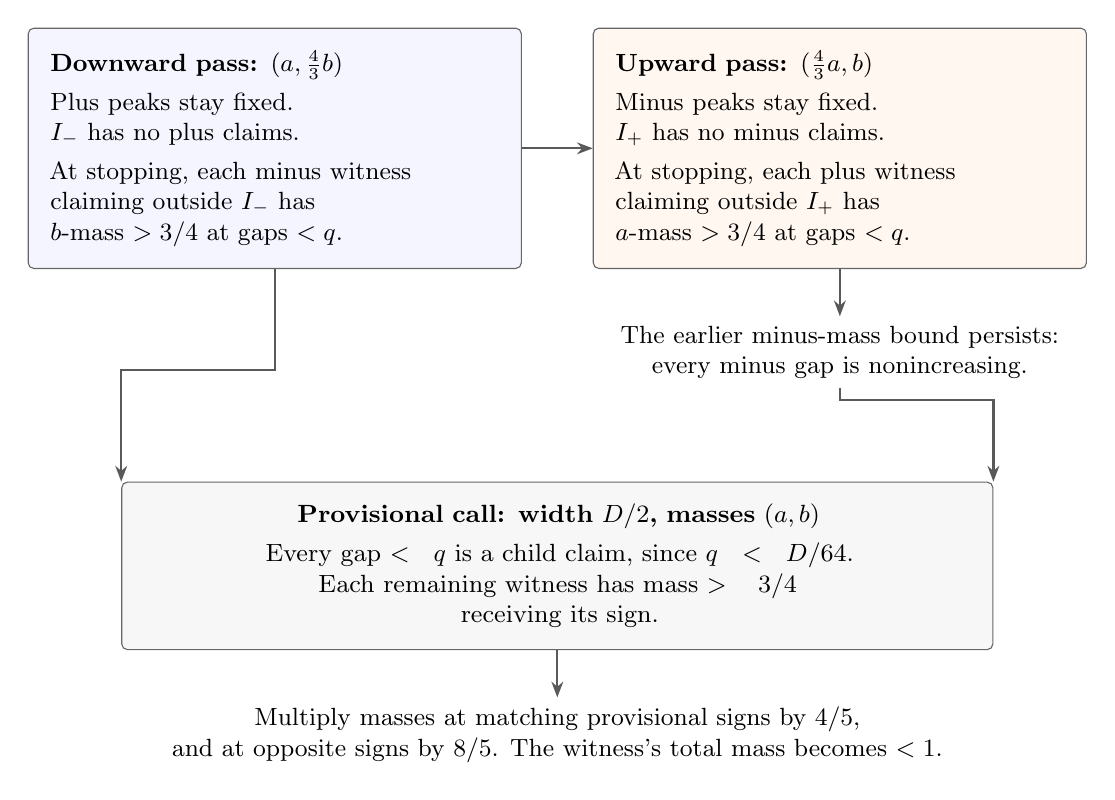
\begin{tikzpicture}[
  font=\small,
  stage/.style={draw=black!60,rounded corners=2pt,align=left,
    text width=5.7cm,inner sep=8pt},
  flow/.style={-{Stealth[length=2mm]},thick,draw=black!65}
]
\node[stage,fill=blue!4] (down) at (0,0) {
  \textbf{Downward pass: $(a,\frac43 b)$}\\[3pt]
  Plus peaks stay fixed.\\
  $I_-$ has no plus claims.\\[3pt]
  At stopping, each minus witness\\
  claiming outside $I_-$ has\\
  $b$-mass $>3/4$ at gaps $<q$.
};
\node[stage,fill=orange!6,right=9mm of down] (up) {
  \textbf{Upward pass: $(\frac43 a,b)$}\\[3pt]
  Minus peaks stay fixed.\\
  $I_+$ has no minus claims.\\[3pt]
  At stopping, each plus witness\\
  claiming outside $I_+$ has\\
  $a$-mass $>3/4$ at gaps $<q$.
};
\draw[flow] (down.east) -- (up.west);
\node[align=center,font=\small,below=6mm of up] (persist)
  {The earlier minus-mass bound persists:\\
   every minus gap is nonincreasing.};
\draw[flow] (up.south) -- (persist.north);
\node[stage,text width=10.5cm,align=center,fill=black!3,
  below=27mm of $(down.south)!0.5!(up.south)$] (wide) {
  \textbf{Provisional call: width $D/2$, masses $(a,b)$}\\[3pt]
  Every gap $<q$ is a child claim, since $q<D/64$.\\
  Each remaining witness has mass $>3/4$\\
  receiving its sign.
};
\draw[flow] (down.south) -- ++(0,-1.28) -| (wide.north west);
\draw[flow] (persist.south) -- ++(0,-.15) -| (wide.north east);
\node[align=center,below=6mm of wide] (last) {
  Multiply masses at matching provisional signs by $4/5$,\\
  and at opposite signs by $8/5$.  The witness's total mass becomes $<1$.
};
\draw[flow] (wide.south) -- (last.north);
\end{tikzpicture}

 \caption{The two passes preserve opposite peaks and force opposite
 mass inequalities.  A remaining witness means one with a claim
 outside its own override set: $I_+$ for plus witnesses and $I_-$
 for minus witnesses.  The upward pass preserves the mass inequality
 obtained during the downward pass.}
 \label{fig:labeling-passes}
\end{figure}

\subsection{Mass reweighting and completion of the proof}

\begin{proof}[Proof of Theorem~\ref{thm:labeling}]
Termination follows from Lemma~\ref{lem:label-rank}; we prove the
labeling guarantee by induction on the same rank.  In the mass
base case, an index labeled $+$ has $b_i>1$, so no minus witness
can contain that index in its support or claim it.  At an index
labeled $-$ one has $b_i\le1$ and $a_i b_i>1$, hence $a_i>1$;
no plus witness can claim that index.  This proves both guarantees.

In the width base case, Lemma~\ref{lem:label-comparison} gives
$y\le t^*\le z$ for all witnesses.  A plus claim forces
$t_i^*\ge u_i-P>A_i+D/2$; a minus claim forces
$t_i^*\le A_i+P<A_i+D/2$.  Thus the returned signs are correct.

For a nonbase call, assume correctness of all its children.  Let
$Q_+=\{i:\ell_i^0=+\}$ and $Q_-=\{i:\ell_i^0=-\}$ be the
provisional sign sets.  Consider a plus witness $y$ that has a
claim outside $I_+$.  By Equation~\eqref{eq:label-final-plus-mass},
the set $G_y=\{i:g_i^y(k^f)<q\}$ has $a$-mass greater than
$3/4$.  It lies in $S_y$ by Lemma~\ref{lem:label-translation}.
Apply that lemma with width $r=D/2$ to the provisional call.
Its plus masses are unchanged, so the translated vector is a
plus witness.  Since
\[
 q=D/128<D/64=r/32,
\]
every index in $G_y$ is a claim of this translated witness.
All these indices belong to $Q_+$ by the child's guarantee.
Consequently
\begin{equation}
 \bar a(S_y)
   =\frac85 a(S_y)-\frac45 a(S_y\cap Q_+)
   <\frac85-\frac45\cdot\frac34=1.
 \label{eq:label-plus-survives}
\end{equation}
The parent vector $y$ is still a subsolution in the unchanged box,
so it is a plus witness for the continuation.

For a minus witness $z$ having a claim outside $I_-$, the set
$G_z=\{i:g_i^z(k^f)<q\}$ has $b$-mass greater than $3/4$ by
Equation~\eqref{eq:label-final-minus-mass}.  It lies in $S_z$.
The width-$D/2$ minus translation is a witness for the provisional
call because the minus masses are unchanged; every index in $G_z$
is one of its claims, and hence belongs to $Q_-$.  Therefore
\begin{equation}
 \bar b(S_z)
   =\frac85 b(S_z)-\frac45 b(S_z\cap Q_-)
   <\frac85-\frac45\cdot\frac34=1.
 \label{eq:label-minus-survives}
\end{equation}
The same vector $z$ is a minus witness for the continuation.

It remains to check every claim after the overrides.  Let $y$
claim $i$.  Lemma~\ref{lem:label-down} gives $i\notin I_-$.
If $i\in I_+$, it receives the plus override.  If $i\notin I_+$,
Equation~\eqref{eq:label-plus-survives} applies to $y$, the
continuation labels $i$ by $+$, and no override changes it.
Now let $z$ claim $i$.  Lemma~\ref{lem:label-up} gives
$i\notin I_+$.  If $i\in I_-$, it receives the minus override.
Otherwise Equation~\eqref{eq:label-minus-survives} applies to $z$,
and the continuation's minus label is unchanged.  In particular
$I_-\cap I_+$ contains no claim of either sign, so the stated
priority between overrides causes no conflict.  This completes
the induction.
\end{proof}

\section{From labels to an exact decision}
\label{sec:application}

We now apply Theorem~\ref{thm:labeling} to a scaled discounted map.
The labels need not locate its fixed point directly. Instead, we construct
two integer comparison vectors on opposite sides of that point. Their
coordinatewise distance is small, so a label excluding one vector from a
boundary strip also allows that boundary to move past a smaller strip
without excluding either vector. Repeating this operation gives the
accuracy required by Theorem~\ref{thm:discount}.

\subsection{Two nearby integer comparison vectors}

Use the integers $W,Q,A_0,H$ of Section~\ref{sec:discount}, and set
\begin{equation}
\begin{gathered}
 N=32H^2,\qquad \lambda=1/N=\lambda_0,\qquad \gamma=1-1/N,\\
 K=256(N+1),\qquad S=16HK,\qquad J=SW+N+1.
\end{gathered}
\label{eq:application-parameters}
\end{equation}
Let
\[
 F(t)=S f_\lambda(t/S),\qquad x=S v(\lambda).
\]
Then $F(x)=x$, the map $F$ is monotone, and
\begin{equation}
 F(t+c\one)=F(t)+\gamma c\one\qquad(t\in\R^n,\ c\in\R).
\label{eq:application-shift}
\end{equation}
Thus $F$ has the properties used in Section~\ref{sec:labeling}.
Define the integer vectors
\begin{equation}
 Y=\lfloor x\rfloor-N\one,
 \qquad Z=\lceil x\rceil+N\one.
\label{eq:comparison-vectors}
\end{equation}
Floors and ceilings are coordinatewise; in particular, a floor of a
negative number is taken toward minus infinity. These vectors are used
only in the proof. The algorithm will not compute them.

\begin{lemma}
\label{lem:comparison-vectors}
The vectors in \eqref{eq:comparison-vectors} satisfy
\[
 F(Y)\ge Y,\qquad F(Z)\le Z,\qquad Y\le x\le Z,
 \qquad \|Y\|_\infty,\|Z\|_\infty\le J.
\]
For every coordinate $i$,
\begin{equation}
 Z_i-Y_i\le 2(N+1)=K/128.
\label{eq:comparison-gap}
\end{equation}
\end{lemma}
\begin{proof}
The inequalities
$x-(N+1)\one\le Y\le x-N\one$ and
$x+N\one\le Z\le x+(N+1)\one$, together with
$\gamma(N+1)=N-1/N\le N$, give
\[
 F(Y)\ge x-\gamma(N+1)\one\ge x-N\one\ge Y
\]
and
\[
 F(Z)\le x+\gamma(N+1)\one\le x+N\one\le Z.
\]
Here we used monotonicity and \eqref{eq:application-shift}.
The remaining conclusions follow from these defining bounds and
$\|x\|_\infty\le SW$.
\end{proof}

\subsection{Shrinking the box}

Recall that the permitted widths are $D=h2^d$ with
$128\le h\le255$ and integers $d\ge0$. Start with
\begin{equation}
 A=-J\one,\qquad D=D_0=128\cdot2^{d_0},
 \label{eq:initial-box}
\end{equation}
where $d_0$ is the least nonnegative integer for which $D_0\ge2J$.
The box $[A,A+D\one]$ contains $Y$ and $Z$.

While $D>K$, call $\cL(A,D,a,b)$ with
$a_i=b_i=1/n$ for all $i$. Put $u=A+D\one$ and $P=D/32$.
Within the current box, $Y$ is a subsolution and $Z$ is a
supersolution, and their support masses are at most one. Consequently,
the labeling guarantee has the following contrapositive form:
\begin{equation}
 \begin{aligned}
 \text{label }+\text{ at }i&\quad\Longrightarrow\quad Z_i>A_i+P,\\
 \text{label }-\text{ at }i&\quad\Longrightarrow\quad Y_i<u_i-P.
 \end{aligned}
 \label{eq:label-exclusions}
\end{equation}
For example, $Z_i\le A_i+P$ would be a minus claim and would require
a minus label.

Let $D'$ be the next smaller permitted width. More explicitly,
\begin{equation}
 D'=\begin{cases}
 (h-1)2^d,&h>128,\\
 255\cdot2^{d-1},&h=128.
 \end{cases}
 \label{eq:next-width}
\end{equation}
The second case has $d\ge1$, because the loop condition implies
$D>K>255$. Set $\delta=D-D'$. In the first case
$\delta/D=1/h\le1/128$; in the second case this ratio is $1/256$.
Thus
\begin{equation}
 0<\delta\le D/128,
 \qquad Z_i-Y_i\le K/128<D/128.
 \label{eq:shrink-slack}
\end{equation}
Define
\[
 A'_i=\begin{cases}
 A_i+\delta,&\text{if the label is }+,\\
 A_i,&\text{if the label is }-.
 \end{cases}
\]
Replace $(A,D)$ by $(A',D')$.

\begin{lemma}
\label{lem:box-invariant}
Every box in this iteration contains $Y$ and $Z$. The iteration makes
at most $128(d_0+1)$ calls to $\cL$ and ends with $D\le K$.
\end{lemma}
\begin{proof}
The initial containment was established above. At a plus coordinate,
\eqref{eq:label-exclusions} and \eqref{eq:shrink-slack} give
\[
 Y_i>Z_i-D/128>A_i+D/32-D/128
       =A_i+3D/128\ge A_i+\delta.
\]
The lower endpoint can therefore increase by $\delta$; the upper
endpoint remains unchanged. At a minus coordinate the same inequalities
give
\[
 Z_i<Y_i+D/128<u_i-D/32+D/128
       =u_i-3D/128\le u_i-\delta.
\]
The upper endpoint can decrease by $\delta$; the lower endpoint remains
unchanged. This proves the induction step for both comparison vectors.

There are only $128$ permitted mantissas at any exponent, and the
exponent never increases. The strictly decreasing sequence of widths
therefore has at most $128(d_0+1)$ terms before reaching the stopping
range, which contains all permitted widths at exponent zero.
\end{proof}

At termination, $Y\le x\le Z$ and the invariant imply
$A_i\le x_i\le A_i+D$. Hence
\begin{equation}
 \left|\frac{A_i}{S}-v_i(\lambda)\right|
 \le\frac KS=\frac1{16H}.
 \label{eq:fixedpoint-error}
\end{equation}
Theorem~\ref{thm:discount} now gives
\begin{equation}
 \left|\frac{A_i}{S}-\val(i)\right|\le\frac1{8H}.
 \label{eq:final-error}
\end{equation}
Output exactly the indices satisfying
\begin{equation}
 \frac{A_i}{S}\ge-\frac1{2H},
 \quad\text{equivalently}\quad A_i\ge-8K.
 \label{eq:output-test}
\end{equation}
If $\val(i)=0$, \eqref{eq:final-error} puts $A_i/S$ at least
$-1/(8H)$, so the index is included. If $\val(i)>0$, the same conclusion
holds. If $\val(i)<0$, the value gap in Theorem~\ref{thm:discount}
gives $A_i/S\le-1/H+1/(8H)=-7/(8H)$, so the index is excluded.
This proves exact correctness, including equality at zero.

\subsection{Bit complexity and uniformity}
\label{subsec:bit-complexity}

It remains to show that the potentially large integer widths do not
produce a large recursion tree, and that every local computation has
polynomial bit cost. The first point uses the mass-product rank of
Section~\ref{sec:labeling}; the second uses the explicit binary encoding.

Since every vertex has an outgoing edge and the input is explicit,
$n,|E|=O(L+1)$. The binary lengths of the probabilities and rewards give
\[
 \log_2 Q=O(L+1),\qquad \log_2 W=O(L+1),\qquad
 \log_2 A_0=O((L+2)^2).
\]
In particular, all integers in \eqref{eq:application-parameters} and
\eqref{eq:initial-box} have $O((L+2)^2)$ bits, and
$d_0=O((L+2)^2)$. Reading the input and forming these integers by ordinary
exact arithmetic take polynomial time. Every recursive box lies in its
parent, and every outer box lies in the initial box. Thus all box
endpoints, pivot coordinates, and integer arguments to $F$ have
polynomial binary length.

For an integer vector $t$, the quantities used to evaluate $F_i(t)$ are
\begin{equation}
 \frac{S w(e)+(N-1)t_j}{N},\qquad e:i\longrightarrow j.
 \label{eq:exact-evaluation}
\end{equation}
Max and Min take exact extrema. At a chance vertex write the encoded
probability as $p(e)=c_e/d_e$ with $d_e>0$. Its weighted sum can be
formed with the common denominator $QN$ and integer numerator
\[
 \sum_{e:i\to j}c_e\frac{Q}{d_e}
           \bigl(Sw(e)+(N-1)t_j\bigr).
\]
Every $d_e$ divides $Q$, even when input fractions are not reduced.
This formula gives polynomial bit lengths and polynomial bit cost for
an evaluation and its coordinatewise floors. Zero probabilities and
parallel edges require no special handling.

Consider one outer call, whose initial masses are $a_i=b_i=1/n$.
For a recursive call put
\[
 \mu=\min_i a_i b_i,\qquad \rho=\frac{32}{25},\qquad
 B(\mu)=\min\{j\in\Z_{\ge0}:\rho^j\mu>1\}.
\]
The initial value $B_0=B(1/n^2)$ is $O(\log(n+1))$; this includes
$n=1$, for which $B_0=1$. Every recursive edge decreases $d+B$.
Only the provisional-label child can preserve $B$, and it decreases
$d$ by one. Each other child decreases $B$ by at least one and does
not increase $d$. Thus the depth is at most
\[
 \Lambda=d_0+B_0,
\]
and any root-to-node path contains at most $B_0$ edges decreasing $B$.
At each node there is at most one $B$-preserving child and at most
\[
 s_*=2(1024n+1)+1=2048n+3
\]
other children: the two pivot passes account for the first term and
the reweighted call for the final one.

A path of length $\ell$ with $j$ edges decreasing $B$ is specified by
their $j$ positions and at most $s_*$ choices at each such position;
the other child, if present, is unique. The total number of nodes is
therefore at most
\begin{align}
 \sum_{\ell=0}^{\Lambda}\sum_{j=0}^{\min(\ell,B_0)}
       \binom{\ell}{j}s_*^j
 &\le (\Lambda+1)(B_0+1)(1+\Lambda s_*)^{B_0} \\
 &=2^{O((\log_2(L+2))^2)}.
 \label{eq:tree-bound}
\end{align}
The distinction between these two kinds of children is essential:
the depth may be polynomial in $L$, but branching choices occur only
$O(\log(n+1))$ times on any path.

All masses can be stored as unreduced positive fractions. An edge that
changes masses multiplies each by one of a fixed set of rational
constants, and so increases its numerator and denominator lengths by
at most a constant. The other edge leaves masses unchanged. Thus the
mass lengths are polynomial (indeed $O(\log(n+1))$), and every comparison,
update, and support-independent base test has polynomial bit cost.
The algorithm does not compute $B$; it is used only for this analysis.

Outside its children, a nonbase call performs $O(n+1)$ pivot updates
and associated vector operations, all of polynomial bit cost. In a
width base case, $d<12$ gives $D\le255\cdot2^{11}$, an absolute
constant, so the clipped-floor iteration uses at most $1+nD$
polynomial-cost evaluations. The mass base case is also polynomial.
Consequently \eqref{eq:tree-bound} bounds the bit cost of one outer
call up to a polynomial factor. Lemma~\ref{lem:box-invariant} bounds
the number of outer calls by a polynomial as well.

Finally, all loops, tie rules, integer operations, and recursive calls
are specified by finite algorithms independent of the input. A
depth-first implementation stores a stack of polynomial depth whose
individual records have polynomial length. Scanning such a stack or
copying a record on a deterministic Turing machine costs at most a
polynomial factor per local operation. The final integer tests
\eqref{eq:output-test} and the output take polynomial time.
Absorbing these factors into \eqref{eq:tree-bound} proves the bound
$2^{C(\log_2(L+2))^2}$ for one absolute constant $C$. This completes
the proof of Theorem~\ref{thm:main}.

\begingroup
\small
\setlength{\bibsep}{5pt}
\bibliographystyle{plainnat}
\bibliography{references}
\endgroup
\end{document}
